\subsection{Gehäuse}\label{sec:Gehäuse}
Damit die Tests in einer hochwertigen Umgebung durchgeführt werden können, ist ein professionelles Gestell der Grundstein für eine ausgezeichnete Teststation. Dadurch der Korpus stabil, leicht, einfach transportierbar und optisch bewundernswert sein sollte, wurden uns von der Robotunits GmbH 40x40 Alu Profile\autocite{alu} zu Verfügung gestellt. Diese Profile sind universell einsetzbar, erfüllen unsere Ansprüche und können so eine perfekte Basis für unsere Teststation bilden. \\
\vspace{3mm}
Die Profile werden mit einem Gewinde Stirnseitig geliefert. An den Gewinde werden sogenannten 90° Verbinder\autocite{Verbinder} montiert, denn so kann man die verschiedenen Teile einfach zusammenschrauben.\\
\vspace{3mm}
\begin{figure}[H]
    \centering
    \begin{subfigure}[b]{0.4\textwidth}
        \centering
        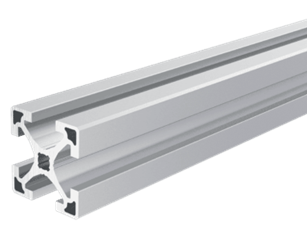
\includegraphics[width=\textwidth]{image/profil.png}
        \caption{Profil}
        \label{fig:bild1}
    \end{subfigure}
    \hfill
    \begin{subfigure}[b]{0.2\textwidth}
        \centering
        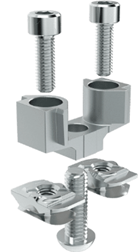
\includegraphics[width=\textwidth]{image/profil2.png}
        \caption{Verbinder}
        \label{fig:bild2}
    \end{subfigure}
    \caption{Profil und Verbinder}
    \label{fig:zwei_bilder}
\end{figure}
\pagebreak

Das Gestell wird in drei Bereiche aufgeteilt:\\
\begin{itemize}
    \item Bedienfläche
    \begin{itemize}
        \item Die oberste Fläche wird als Arbeitsfläche für den Anwender verwendet. Auf dieser Fläche kann ein Bildschirm oder ein Laptop platziert werden, und von dort aus die  die Tests steuern und die Daten auszulesen.
    \end{itemize}
    \item Testkammer
    \begin{itemize}
        \item In der mittleren Ebene wird eine Kammer gebaut, in der die Tests durchgeführt werden können. Dieser Bereich bekommt Wände aus PVC Platten und kann mit einer Tür verschlossen werden. Darin wird ein Gyroskop, Sensoren, eine Lampe und sonstige Hardwareteile platziert.
    \end{itemize}
    \item Steuereinheit
    \begin{itemize}
        \item In dem untersten Bereich werden die Steuerungsgeräte platziert wie zum Beispiel der Raspberry, Netzteile, Treiber und sonstige Ansteuerungsgeräte. Dieser Bereich wird mit Plexiglas als Wände verschlossen um von Staub und sonstigen Einwirkungen zu schützen. 
    \end{itemize}
\end{itemize}
\begin{figure}[H]
    \centering
    \includegraphics{image/Skizzegehäuse.png}
    \caption{Skizze Gestell}
    \label{fig:enter-label}
\end{figure}
\pagebreak
Maße der Profile:\\
\vspace{3mm}
Die Maße wurden so gewählt, dass das Gestell eine Grundfläche von 78x78cm hat. Diese Fläche ist groß genug, um einen 27 Zoll Monitor einfach zu platzieren. Die Vertikalen Profile haben eine Länge von 100cm, denn so wird mit den Rollen eine Gesamthöhe von 110cm erreicht. Diese Höhe gewährleistet eine gesunde und komfortable Arbeitshöhe.\\                                       \vspace{3mm}  
Das Gewicht vom Gesamtgestellt aus den Aluprofilen, Rollen und Verbindungen beträgt 22kg.\\
\vspace{3mm}
Für das Gestell sind folgende Teile nötig:
\begin{table}[H]
    \centering
    \begin{tabular}{ | c | c | } 
  \hline
   \textbf{Bezeichnung} & \textbf{Stückzahl}\\ 
  \hline
   70cm Aluminiumprofil 40x40mm & 14\\ 
  \hline
   100cm Aluminiumprofil 40x40mm & 4 \\ 
  \hline
  Stirnverbinder 40x40mm & 28 \\ 
  \hline
  Einschwenkmutter M8 & 30 \\ 
  \hline
  Rollen mit Rückenloch fixierbar & 2 \\ 
  \hline
  Rollen mit Rückenloch & 2 \\ 
  \hline
  Abdeckkappe 40x40mm & 4 \\ 
  \hline
\end{tabular}
    \caption{Stückliste Gestell}
\end{table}

\subsubsection{Holzplatte}
Die verschiedenen Bereiche der Teststation werden mittels  3 Schicht Holzplatten, die eine Stärke von 18mm haben, getrennt. Diese Platten haben die Vorteile, dass sie sehr formstabil und langlebig sind. Außerdem weisen sie dank drei Schichten Massivholz eine hohe Biegefestigkeit. Dankensweise wurden uns die Platten von der Firma Tschabrun Herman Gesellschaft m.b.H. gesponsert. Da die Grundfläche vom Gestell die Fläche von 78x78cm hat, wird aus optischen Gründen die Arbeitsfläche mit den Maßen von 82x82cm gewählt. So steht die Platte auf jeder Seite 2cm über das Alugestell. Damit die Platten in der mittleren und unteren Ebene bündig mit dem Gestell sind, haben diese ein Maß von 78x78cm. Bei diesen Platten müssen die Ecken ausgesägt werden, damit sie formschlüssig mit dem Gestell sind. Diese Aussparungen sind 4x4cm groß, genauso groß wie die Aluprofile. 
\vspace{5mm}
\begin{figure}[H]
    \centering
    \begin{subfigure}[b]{0.4\textwidth}
        \centering
        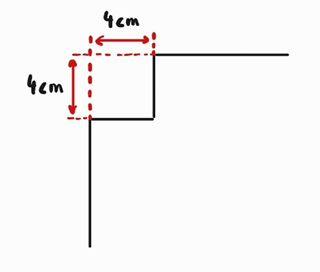
\includegraphics[width=\textwidth]{image/Bild1holzplatte.png}
        \caption{Aussparung Maße}
        \label{fig:bild1}
    \end{subfigure}
    \hfill
    \begin{subfigure}[b]{0.35\textwidth}
        \centering
        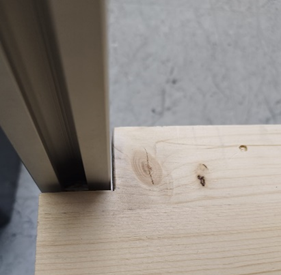
\includegraphics[width=\textwidth]{image/Bild2holzplatte.png}
        \caption{Aussparung umgesetzt}
        \label{fig:bild2}
    \end{subfigure}
    \caption{Aussparung}
    \label{fig:zwei_bilder}
\end{figure}
Damit die Wände befestigt werden können, werden in eine Holzplatte Nuten gefräst. So können die Platten nicht mehr verschoben werden und können fest verklebt werden. Die Nut ist 5mm tief und 8mm breit. Auf der Vorderseite, wird ein Stahlrahmen befestigt,  der auch in eine Nut eingelassen wird, diese Nut ist jedoch 4mm breit und 5mm tief. 
\vspace{5mm}
\begin{figure}[H]
    \centering
    \begin{subfigure}[b]{0.4\textwidth}
        \centering
        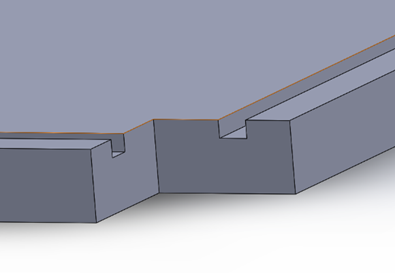
\includegraphics[width=\textwidth]{image/Bild1nut.png}
        
        \label{fig:bild1}
    \end{subfigure}
    \hfill
    \begin{subfigure}[b]{0.41\textwidth}
        \centering
        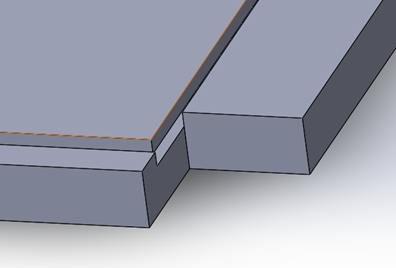
\includegraphics[width=\textwidth]{image/Bild2nut.png}
        
        \label{fig:bild2}
    \end{subfigure}
    \caption{Nut Vorderseite}
    \label{fig:zwei_bilder}
\end{figure}
Jede Holzplatte wird mit M8 Schrauben und Nutsteine angeschraubt. Dazu werden 8mm Löcher in die Holzplatten gebohrt und anschließen werden die die Löcher mit einem Senkbohrer gebohrt, dadurch können die Schrauben bündig mit der Platte verschraubt werden. 
\newpage
\subsubsection{PVC-Platten}
In der mittleren Ebene werden Wände montiert, damit die Kammer luft- und staubdicht ist. Dazu eignen sich Hart PVC-Platten mit einer Dicke von 8mm. Die Platten sind elektrisch gut isoliert, haben eine große Beständigkeit gegen Chemikalien, sind hitzebeständig bis 60°C  und außerdem sorgen sie für ein einzigartiges Design unsere Teststation. Die Platten werden mit einem Pattex Montagekleber verklebt, denn dieser Kleber ist speziell geeignet für PVC- Materialien und überzeugt mit einem sehr starken Halt. 
\vspace{5mm}
\begin{table}[H]
    \centering
    \begin{tabular}{ | c | c | } 
  \hline
   \textbf{Bezeichnung} & \textbf{Stückzahl}\\ 
  \hline
   Hart PVC Schwarz 80x56cm & 3\\ 
  \hline
   Pattex Montagekleber & 2 \\ 
  \hline
\end{tabular}
    \caption{Stückliste PVC-Platte}
\end{table}

Die PVC-Platten werden in die Nut der Aluprofile gesteckt. Da oben die Querstangen mit Verbindungen ausgestattet sind, behindern diese die PVC-Platten. Aus diesem Grund muss jeweils in den Ecken eine 1x2cm Aussparung entfernt werden. 
\subsubsection{Tür}
Es soll möglich sein, die Kammer zu verschließen, um äußerliche Einwirkungen zu verhindern. Zusätzlich sollte die Kammer luftdicht sein, denn weder warme oder kalte Luft sollte entfliehen können. Da auch das Gyroskop akustisch etwas laut ist, dient die Tür auch als Geräusch Verminderung. 
Der Rahmen für die Tür wird aus Holzleisten gefertigt, die eine Stärke von 2cm und eine breite von 4cm haben.\\
\vspace{3mm}
\begin{table}[H]
    \centering
    \begin{tabular}{ | c | c | } 
  \hline
   \textbf{Bezeichnung} & \textbf{Stückzahl}\\ 
  \hline
   Holzleiste 4x2x70cm & 2\\ 
  \hline
   Holzleiste 4x2x56cm & 2 \\ 
  \hline
  Holzleiste 0.2x54x68cm & 1\\
  \hline
  Edelstahlgriff Lochabstand 128mm & 1\\
  \hline
  M3 Schraube mm & 2\\
  \hline
  M3 Mutter & 2\\
  \hline
  Silikon Kleber & 1\\
  \hline
\end{tabular}
    \caption{Stückliste Tür}
\end{table}
\newpage
Die Holzleisten werden auf Gehrung verbunden, denn durch diese Methode vergrößert sich die Kontaktfläche und die Stabilität wird erhöht. 
Plexiglas ist ein transparentes Kunststoffmaterial, das als Ersatz für Glas verwendet wird. Es ist leichter, günstiger und bruchsicherer als Glas. Das Plexiglas hat eine Stärke von 2mm und wird in eine Nut im Rahmen eingelassen, um eine einfache Befestigung zu gewährleisten.  \\
\vspace{3mm}
Zusammenbau:
Um sicherzustellen, dass das Plexiglas während des Zusammenbauens und Verleimens ordnungsgemäß in den Rahmen eingesetzt wurde, waren folgende Schritte erforderlich:\\
\vspace{3mm}
1. Vorbereutung der Leisten
\begin{itemize}
    \item ˆ Zunächst wurde eine lange Leiste mit der Nut nach unten auf die Arbeitsfläche (Fläche X) gelegt.
    \item Eine kurze Leiste mit der Nut nach unten wurde bündig an der rechten Seite der langen Leiste platziert. Dieser Schritt wurde auch auf der linken Seite der langen Leiste mit einer weiteren kurzen Leiste wiederholt.
\end{itemize}
2. Fixierung mit Klebeband:
\begin{itemize}
    \item Die drei Leisten wurden mit Klebeband zusammengehalten, um zu verhindern, dass sie beim Verleimen verrutschen.
\end{itemize}
\vspace{3mm}
3. Vorbereitung für den Leimauftrag:
\begin{itemize}
    \item Die drei Leisten wurden zusammen um 180° gedreht. Holzleim wurde großzügig auf die Oberfläche aufgetragen und gleichmäßig verteilt.
\end{itemize}

4. Einsetzen des Plexiglases:
\begin{itemize}
    \item Das Plexiglas wurde vorsichtig in die Nut der langen Leiste eingelegt. Hierbei konnte eine zweite Person von Vorteil sein, um das Plexiglas zu halten, während die anderen beiden Leisten um 90° angehoben wurden. Dabei wurde darauf geachtet, dass das Plexiglas auch in den kurzen Leisten eingespannt war.
\end{itemize}

5. Abschluss des Rahmens:
\begin{itemize}
    \item Abschließend wurde die verbleibende zweite lange Leiste auf die kurzen Seiten und das Plexiglas gelegt.
\end{itemize}
\newpage
6. Fixierung und Trocknung:
\begin{itemize}
    \item Schraubzwingen wurden verwendet, um den Rahmen fest zusammenzuspannen und den Leim trocknen zu lassen.
Durch diese Schritte wurde sichergestellt, dass das Plexiglas ordnungsgemäß in den Rahmen eingesetzt wurde und während des Verleimens nicht verrutschte.Mit einem Silikonkleber wird das Plexiglas mit der Nut verklebt und verdichtet. Nachdem das Silikon ausgetrocknet war, war die Tür dicht.
Als Türgriff wird ein Edelstahlgriff mit einem Lochabstand von 13cm verwendet. Der Griff kann dank einer soliden Verschraubung sicher und stabil angebracht werden, was eine zuverlässige Nutzung gewährleistet.
Die Tür wird mit einfachen Scharnieren an dem Gestell befestigt.
\end{itemize}



\subsubsection{Dichtungsrahmen}
Damit man die Tür dicht verschließen kann und diese einen Anschlag hat, braucht es einen Rahmen. Der Rahmen wird aus 4mm dickem und 35mm breiten Flachstangen erstellt. Auf diesen Rahmen kommt ein Dichtungsband und die Tür wird dann mit sogenannten Kniehebelspanner an den Rahmen gedrückt. So ist es möglich, die Kammer Luft und Staubdicht zu verschließen. Der Rahmen wird an den Seiten an das Gestell geklebt und unten sowie oben in eine Nut eingelassen.
\vspace{5mm}
\begin{table}[H]
    \centering
    \begin{tabular}{ | c | c | } 
  \hline
   \textbf{Bezeichnung} & \textbf{Stückzahl}\\ 
  \hline
   Flachstange 35x580mm & 2\\ 
  \hline
   Flachstange 20x664mm & 1 \\ 
  \hline
  Flachstange 35x664mm & 1 \\ 
  \hline
  Schaumisolierung 3m & 1 \\ 
  \hline
\end{tabular}
    \caption{Stückliste Dichtungsrahmen}
\end{table}
\vspace{5mm}
\begin{figure}[H]
    \centering
    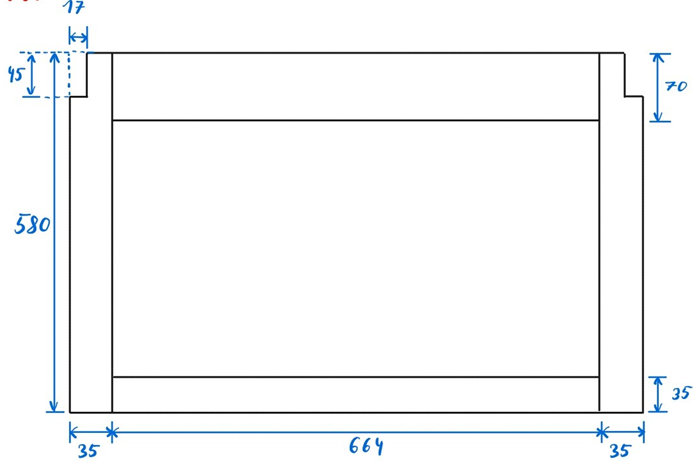
\includegraphics[scale=1.2]{image/skizzerahmen.png}
    \caption{Skizze Dichtungsrahmen in mm}
    \label{fig:enter-label}
\end{figure}
Die Flachstangen werden zusammengeschweißt und dann mit einem Tiefschwarz Lackspray lackiert. Das Dichtungsband wird doppelt mit einem Abstand dazwischen auf den Rahmen geklebt. \\
Das Schaumisolierbar hat eine hervorragende Dicht- und Verformungsbeständigkeit, ist für Temperaturen von -50°C bis 150°C geeignet, hat eine gute Dämpfung sowie eine gute Wärmeisolierung.
\begin{figure}[H]
    \centering
    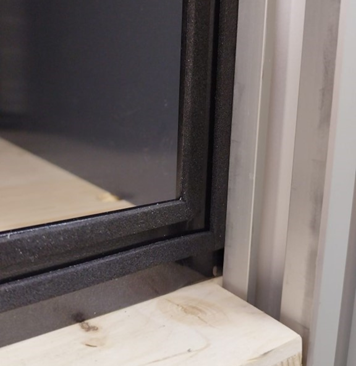
\includegraphics{image/rahmen2.png}
    \caption{Bild Rahmen}
    \label{fig:enter-label}
\end{figure}
\vspace{5mm}

\subsubsection{Schließer}
Damit die Kammer fest verschlossen werden kann, wird die Tür mit sogenannten Kniehebelspanner an den Rahmen gepresst.
Die Kniehebelspanner können nicht direkt am Gestell montiert werden, da ihr Arm zu lang ist und dadurch die Tür nicht mehr geöffnet werden könnte.
\begin{figwindow}[0,r,\includegraphics[scale=1]{image/Schließer1.png},{Schließer}]
Aus diesem Grund wurde aus einem Reststück Aluprofil ein Adapter gebaut und mit einem 3D Drucker ein Winkel gedruckt. In das Loch vom Aluprofil wurde ein Gewinde geschnitten, denn so kann man den Winkel anschrauben.
\end{figwindow}
\vspace{20mm}
\begin{figwindow}[0,l,\includegraphics[scale=1]{image/Schließer2.png},{Winkel}]
Damit der Winkel genau auf das Aluprofil passt, hat dieser eine Grundfläche von 4x4cm. Die Rückseite wird an dem Gestell mit einer M8 Schraube fixiert.
\end{figwindow}
\vspace{40mm}
\begin{figure}[H]
    \centering
    \begin{subfigure}[b]{0.4\textwidth}
        \centering
        \includegraphics[width=\textwidth]{image/geöffnet.png}
        \caption{geöffnet}
        \label{fig:bild1}
    \end{subfigure}
    \hfill
    \begin{subfigure}[b]{0.45\textwidth}
        \centering
        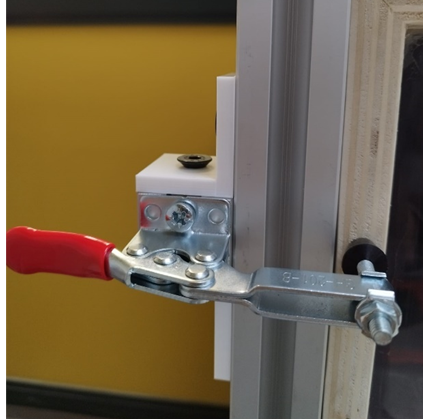
\includegraphics[width=\textwidth]{image/geschlossen.png}
        \caption{geschlossen}
        \label{fig:bild2}
    \end{subfigure}
    \caption{Zustand Schließer}
    \label{fig:zwei_bilder}
\end{figure}